%%%%%%%%%%%%%%%%%%%%%%%%%%%%%%
%% ESTRUCTURA DEL DOCUMENTO %%
%%%%%%%%%%%%%%%%%%%%%%%%%%%%%%

                                                       
% ___  ____ ____ ____ _  _ ___  _  _ _    ____ 
% |__] |__/ |___ |__| |\/| |__] |  | |    |  | 
% |    |  \ |___ |  | |  | |__] |__| |___ |__|


% Define la clase de documento como "man" para el estilo APA con gráficos flotantes dentro del texto
\documentclass[man, floatsintext]{apa7}

% Configura el soporte para el idioma español y el formato de tablas en español
\usepackage[spanish, es-tabla]{babel}

% Permite la codificación UTF-8 para caracteres
\usepackage[utf8]{inputenc}

% Permite insertar figuras usando \placein{figure} en este punto
\usepackage[section]{placeins}

% Configura biblatex para el estilo APA con ordenación por autor, citas nombre-año, backend biber
\usepackage[style=apa,sortcites=true,sorting=nyt,backend=biber]{biblatex}

% Carga el paquete csquotes para un manejo inteligente de comillas
\usepackage{csquotes}

% Carga varios paquetes para tablas, texto verbatim, gráficos y URLs
\usepackage{array,fancyvrb,graphicx,verbatim,xurl}

% PARA GENERAR TEXTO RANDOM
\usepackage{lipsum}  

% (No cambiar)
\title{\titulo}  
\shorttitle{\titulocorto}  
\author{\autor} 
\affiliation{\afiliacion}

% TODO: Comentar para generar el documento completo
%\includeonly{contenido/introduccion}

\begin{document}
	% NOTAS DEL AUTOR
	%%%%%%%%%%%%%%%%%%%%
%% NOTA DEL AUTOR %%
%%%%%%%%%%%%%%%%%%%%

\authornote{
	
	\addORCIDlink{Nombre del Investigador}{0000-0000-0000-0000}
	
	Aquí van las notas del autor.
	
}
	
	% INCLUSIÓN DE DATOS DE RESUMEN / ABSTRACT
	
%____ ___  ____ ___ ____ ____ ____ ___ 
%|__| |__] [__   |  |__/ |__| |     |  
%|  | |__] ___]  |  |  \ |  | |___  |

\abstract{Aquí va el resumen o abstract del documento}

\keywords{Aquí, van, las, palabras, clave, separadas, por, coma}

	
	
	% PORTADA
	\maketitle
	
	
	% OPCIONAL:
	\tableofcontents
	\newpage
	
	% INTRODUCCIÓN
	\section{\titulo}
	
%_ _  _ ___ ____ ____ ___  _  _ ____ ____ _ ____ _  _ 
%| |\ |  |  |__/ |  | |  \ |  | |    |    | |  | |\ | 
%| | \|  |  |  \ |__| |__/ |__| |___ |___ | |__| | \|


\lipsum[2-3] \parencite{Borst2011a}.

	
	
	% METODO
	% MÉTODO %

\section{Método}
\subsection{Un Subtitulo}
\lipsum[1]
\subsubsection{Un Subsubtítulo}
\lipsum[1]

	
	
	% RESULTADOS
	
%____ ____ ____ _  _ _    ___ ____ ___  ____ ____ 
%|__/ |___ [__  |  | |     |  |__| |  \ |  | [__  
%|  \ |___ ___] |__| |___  |  |  | |__/ |__| ___]

\section{Resultados}
\lipsum[1]

\begin{table}[h]
	\caption{Sample Basic Table}
	\label{tab:BasicTable}
	\begin{tabular}{@{}llr@{}}         \toprule
		\multicolumn{2}{c}{Item}        \\ \cmidrule(r){1-2}
		Animal    & Description & Price \\ \midrule
		Gnat      & per gram    & 13.65 \\
		& each        &  0.01 \\
		Gnu       & stuffed     & 92.50 \\
		Emu       & stuffed     & 33.33 \\
		Armadillo & frozen      &  8.99 \\ \bottomrule
	\end{tabular}
\end{table}

\lipsum[1]

\begin{figure}
	\caption{Descripción de figuras.}
	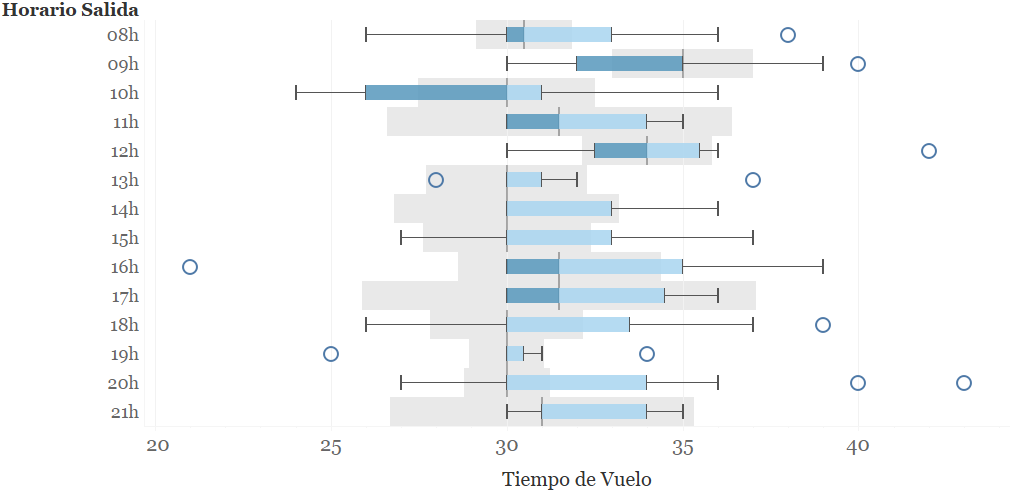
\includegraphics[scale=0.85]{contenido/multimedios/figura1}
	\label{fig:Figure1}
\end{figure}

\lipsum[1]

	
	% DISCUSIÓN
	
%___  _ ____ ____ _  _ ____ _ ____ _  _ 
%|  \ | [__  |    |  | [__  | |  | |\ | 
%|__/ | ___] |___ |__| ___] | |__| | \|


\section{Discusión}
\lipsum[5]
	

	% REFERENCIAS
	\printbibliography	
	
	% OPCIONAL: Notas al Pie de Página o Notas al Final

	% OPCIONAL: Tablas
	
	% OPCIONAL: Figuras
	
	% OPCIONAL: Apendices
	\appendix
	\addcontentsline{toc}{section}{Apéndice A}
	%%%%%%%%%%%%%%%%
%% APÉNDICE A %%
%%%%%%%%%%%%%%%%

\section{Instrumentos}
\label{app:instrumentos}
\lipsum[30]
	\addcontentsline{toc}{section}{Apéndice B}
	%%%%%%%%%%%%%%%%
%% APÉNDICE A %%
%%%%%%%%%%%%%%%%

\section{Data Piloto}
\label{app:datapiloto}
\lipsum[30]
	


\end{document}
